% DO NOT COMPILE THIS FILE DIRECTLY!
% This is included by the other .tex files.

\section{Introdução à Lógica Proposicional} % Necessário para gerar o \tableofcontents

\begin{frame}[t]
\vskip 3cm
\begin{center}
{\Huge Introdução à\\Lógica Proposicional}
\end{center}
\end{frame}

\begin{frame}[t]
	\begin{figure}
		\center{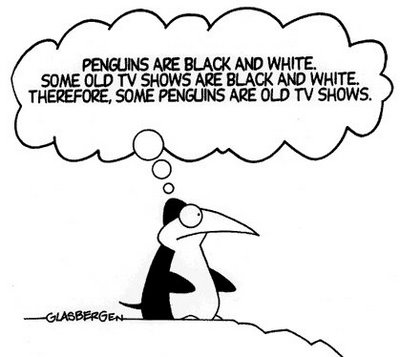
\includegraphics[scale=0.9]{penguins.png}}
	\end{figure}
\end{frame}

\subsection{Definições Básicas}

\begin{frame}[t]{O que é Lógica?} % Título do Frame
\end{frame}

\begin{frame}[t]{O que é Lógica?} % Título do Frame
\begin{center}
``{\it Conhecimento das formas gerais e regras gerais do pensamento correto e verdadeiro, independentemente dos conteúdos pensados; regras para demonstração científica verdadeira; regras para pensamentos não-científicos; regras sobre o modo de expor o conhecimento; regras para verificação da verdade ou falsidade de um pensamento etc.}''
\end{center}

\begin{flushright}
\footnotesize{[Marilena Chaui, ``{\it Convite a Filosofia}'', 2002]}
\end{flushright}
\end{frame}

%\subsection{Conceitos Introdutórios}

\begin{frame}[t]{Conceitos Introdutórios} % Título do Frame
	\begin{itemize}
		\item Proposição
		   \begin{itemize}
		   \item conjunto de palavras ou símbolos que exprimem um pensamento (fatos ou juízos) de sentido completo
		   \item Exemplos
		   \begin{enumerate}
		   \item A Lua é o satélite da Terra
		   \item Recife é a capital de Pernambuco
	              \item $\pi > \sqrt{5}$
	 	   \item $1 + 1 = 3$
		   \end{enumerate}
		   \end{itemize}
		\item Princípios das Proposições
                         \begin{description}
		    \item[Não contradição:] uma proposição não pode ser verdadeira e falsa ao mesmo tempo
  		    \item[Terceiro excluído:] uma proposição é sempre ou verdadeira ou falsa, não existe terceira opção
		    \end{description}
	\end{itemize}
\end{frame}

\begin{frame}[t]{Conceitos Introdutórios} % Título do Frame
	\begin{itemize}
		\item Proposições {\bf Verdadeiras}
		   \begin{enumerate}
	 	   \item $1 + 1 = 2$
		   \item A Lua é o satélite natural da Terra
		   \item Florianópolis e Recife são capitais de estados
		   \end{enumerate}
		\item Proposições {\bf Falsas}
		   \begin{enumerate}
	 	   \item Vasco da Gama descobriu o Brasil
		   \item $3 \times 4 < 100 \div 13$
		   \item $3 \div 5$ é um número inteiro
		   \end{enumerate}
	\end{itemize}
\end{frame}

\begin{frame}[t]{Conceitos Introdutórios} % Título do Frame
	Determine ``V'' ou ``F'' para as afirmações abaixo
	\begin{enumerate}
	  \item O Brasil já ganhou 5 títulos mundiais
	\end{enumerate}
\end{frame}

\begin{frame}[t]{Conceitos Introdutórios} % Título do Frame
	Determine ``V'' ou ``F'' para as afirmações abaixo
	\begin{enumerate}
	  \item O Brasil já ganhou 5 títulos mundiais
	  \item $\pi = 3.14$
	\end{enumerate}
\end{frame}

\begin{frame}[t]{Conceitos Introdutórios} % Título do Frame
	Determine ``V'' ou ``F'' para as afirmações abaixo
	\begin{enumerate}
	  \item O Brasil já ganhou 5 títulos mundiais
	  \item $\pi = 3.14$
	  \item Eu sempre minto
	\end{enumerate}
\end{frame}

\begin{frame}[t]{Conceitos Introdutórios} % Título do Frame
	Determine ``V'' ou ``F'' para as afirmações abaixo
	\begin{enumerate}
	  \item O Brasil já ganhou 5 títulos mundiais
	  \item $\pi = 3.14$
	  \item Eu sempre minto
	\end{enumerate}
	
	\vskip 1cm

	\begin{center}
	{\Huge {\sc Cuidado com paradoxos!}}
	\end{center}
\end{frame}

\begin{frame}[t]{Conceitos Introdutórios} % Título do Frame
	Determine ``V'' ou ``F'' para as afirmações abaixo
	\begin{enumerate}
	  \item O Brasil já ganhou 5 títulos mundiais
	  \item $\pi = 3.14$
	  \item Eu sempre minto
	\end{enumerate}
	
	\vskip 1cm

	\begin{center}
	{\Huge {\sc Cuidado com paradoxos!}} 

	\vskip 1cm

	{\it I don't speak English}

	\end{center}
\end{frame}


\begin{frame}[t]{Função de Avaliação ou Interpretação Lógica} % Título do Frame
	
%\textcolor{red}{Rogério: introduzi este conceito nos
%exemplos anteriores.}\\


\begin{description}

\item[Uma proposição:]   uma proposição $p$ sempre assume $V$ ou $F$.  Nunca os
dois valores simultaneamente, ou nenhum dos dois. 
Sempre é alguma coisa em $V$ ou $F$, logo ...

  \item[Mapeamento Binário:]  $f(p) \to V$ ou  $f(p) \to F$
	
  \item[Função de Avaliação:] $f_{avalia}(p) = \{V, F\}$\\
%Fiz vários exercícios com os alunos sobre isto, interpretando
%proposições.

\item[Função de Avaliação $f(p)$ ou Interpretação Lógica $\Phi(p)$:] $f_{avalia}(p) \equiv \Phi(p)$

\item[Resumindo $f(p)$ ou $\Phi(p)$:] são utilizadas  para especificar o valor final sobre o conjunto
 $\{V, F\}$,   de uma fórmula lógica ou proposição composta



	\end{description}
\end{frame}




\begin{frame}[t]{Conceitos Introdutórios} % Título do Frame
	Alfabeto
	\begin{description}
	  \item[Símbolos Ortográficos:] ( )
	  \item[Constantes Lógicas:] {\em True, False} ({\bf V} e {\bf F} neste curso)
	  \item[Símbolos Proposicionais:] $p, q, r, s, p_1, r_2, \ldots$
	  \item[Conectores:] $\sim (\neg), \wedge, \vee, \rightarrow, \leftrightarrow$
	\end{description}
\end{frame}

\begin{frame}[t]{Conceitos Introdutórios} % Título do Frame
	Fórmulas bem formadas ({\em fbf})
	\begin{itemize}
	  \item Constantes lógicas são fórmulas
	  \item Símbolos proposicionais são fórmulas
	  \item Operação negação: $\sim p$
	  \item Operação conjunção (``e''): $p \wedge q$
	  \item Operação disjunção (``ou''): $p \vee q$
	  \item Operação disjunção exclusiva (``x-ou''): $p\veebar q$
	  \item Operação condicional: $p \rightarrow q$
	  \item Operação bicondicional:$p \leftrightarrow q$
	\end{itemize}
\end{frame}

\begin{frame}[t]{Conceitos Introdutórios} % Título do Frame
	Tabelas-Verdade
	\begin{itemize}
	  \item lista todos os possíveis valores lógicos de uma proposição composta, em função das combinações de todos os possíveis valores para cada proposição simples que a compõe
	  \item Exemplo:  $p \wedge q$
	    \begin{itemize}
	    \item Valores possíveis para ``p'' = V ou F (1 ou 0)
	    \item Valores possíveis para ``q'' = V ou F (1 ou 0)
	   \end{itemize}
	\end{itemize}

	\begin{minipage}[t]{0.45\textwidth}
	\begin{center}	
	\begin{tabular}{|c|c|}
	\hline
	$\mathbf{p}$ & $\mathbf{q}$ \\
	\hline
	V & V \\
	\hline
	V & F \\
	\hline
	F & V \\
	\hline
	F & F \\
	\hline
	\end{tabular}
	\end{center}
	\end{minipage}
	\begin{minipage}[t]{0.45\textwidth}
	\begin{center}	
	\begin{tabular}{|c|c|}
	\hline
	$\mathbf{p}$ & $\mathbf{q}$ \\
	\hline
	0 & 0 \\
	\hline
	0 & 1 \\
	\hline
	1 & 0 \\
	\hline
	1 & 1 \\
	\hline
	\end{tabular}
	\end{center}
	\end{minipage}
\end{frame}

\begin{frame}[t]{Conceitos Introdutórios} % Título do Frame
	Operações Lógicas: {\bf negação} ($\sim$)
	\begin{itemize}
	  \item inversão do valor lógico de uma proposição
	\end{itemize}

	\begin{center}	
	\begin{tabular}{|c|c|}
	\hline
	$\mathbf{p}$ & $\mathbf{\sim p}$ \\
	\hline
	V & F \\
	\hline
	F & V \\
	\hline
	\end{tabular}
	\end{center}
\end{frame}

\begin{frame}[t]{Conceitos Introdutórios} % Título do Frame
	Operações Lógicas: {\bf negação} ($\sim$)
	\begin{itemize}
	  \item Exemplos em Linguagem Natural:
	  \begin{itemize}
	  \item $p:$ O Sol é uma estrela
	  \item $\sim p:$ O Sol não é uma estrela
	  \item $p:$ Carlos é um mecânico
	  \item $\sim p:$ Não é verdade que Carlos é um mecânico
	  \item $\sim p:$ É falso que Carlos é um mecânico
	  \end{itemize}
	\end{itemize}
\end{frame}

\begin{frame}[t]{Conceitos Introdutórios} % Título do Frame
	Operações Lógicas: {\bf conjunção} ($\wedge$)
	\begin{itemize}
	  \item proposição composta que é verdadeira somente quando todas as proposições componentes forem verdadeiras
	\end{itemize}

	\begin{center}	
	\begin{tabular}{|c|c|c|}
	\hline
	$\mathbf{p}$ & $\mathbf{q}$ & $\mathbf{p \wedge q}$ \\
	\hline
	V & V & V \\
	\hline
	V & F & F \\
	\hline
	F & V & F \\
	\hline
	F & F & F \\
	\hline
	\end{tabular}
	\end{center}
\end{frame}

\begin{frame}[t]{Conceitos Introdutórios} % Título do Frame
	Operações Lógicas: {\bf disjunção} ($\vee$)
	\begin{itemize}
	  \item proposição composta que é verdadeira quando pelo menos uma das proposições componentes for verdadeira
	\end{itemize}

	\begin{center}	
	\begin{tabular}{|c|c|c|}
	\hline
	$\mathbf{p}$ & $\mathbf{q}$ & $\mathbf{p \vee q}$ \\
	\hline
	V & V & V \\
	\hline
	V & F & V \\
	\hline
	F & V & V \\
	\hline
	F & F & F \\
	\hline
	\end{tabular}
	\end{center}
\end{frame}

\begin{frame}[t]{Conceitos Introdutórios} % Título do Frame
	Operações Lógicas: {\bf disjunção exclusiva} ($\veebar$)
	\begin{itemize}
	  \item proposição composta que é verdadeira somente quando exatamente uma das proposições componentes for verdadeira
	\end{itemize}

	\begin{center}	
	\begin{tabular}{|c|c|c|}
	\hline
	$\mathbf{p}$ & $\mathbf{q}$ & $\mathbf{p \veebar q}$ \\
	\hline
	V & V & F \\
	\hline
	V & F & V \\
	\hline
	F & V & V \\
	\hline
	F & F & F \\
	\hline
	\end{tabular}
	\end{center}
\end{frame}

\begin{frame}[t]{Conceitos Introdutórios} % Título do Frame
	Operações Lógicas: {\bf condicional} ($\rightarrow$)
	\begin{itemize}
	  \item proposição que representa uma relação do tipo: ``{\bf se p então q}''
	  \item $p$ é chamado {\bf antecedente}
	  \item $q$ é chamado {\bf consequente}
	  \item $\rightarrow$ é chamado operador {\bf implicação}
	\end{itemize}

	\begin{center}	
	\begin{tabular}{|c|c|c|}
	\hline
	$\mathbf{p}$ & $\mathbf{q}$ & $\mathbf{p \rightarrow q}$ \\
	\hline
	V & V & V \\
	\hline
	V & F & F \\
	\hline
	F & V & V \\
	\hline
	F & F & V \\
	\hline
	\end{tabular}
	\end{center}
\end{frame}

\begin{frame}[t]{Conceitos Introdutórios} % Título do Frame
	Operações Lógicas: {\bf condicional} ($\rightarrow$)
	\begin{itemize}
	  \item Exemplos em Linguagem Natural:
	  \begin{itemize}
	  \item Se Maio tem 31 dias então a Terra é plana
	  \item Se $\pi$ é um número real então o Brasil fica na América do Sul
	  \end{itemize}
	\end{itemize}
\end{frame}

\begin{frame}[t]{Conceitos Introdutórios} % Título do Frame
	Operações Lógicas: {\bf bi-condicional} ($\leftrightarrow$)
	\begin{itemize}
	  \item proposição que representa uma relação do tipo: ``{\bf p se e somente se q}''
	\end{itemize}

	\begin{center}	
	\begin{tabular}{|c|c|c|}
	\hline
	$\mathbf{p}$ & $\mathbf{q}$ & $\mathbf{p \leftrightarrow q}$ \\
	\hline
	V & V & V \\
	\hline
	V & F & F \\
	\hline
	F & V & F \\
	\hline
	F & F & V \\
	\hline
	\end{tabular}
	\end{center}
\end{frame}

\begin{frame}[t]{Conceitos Introdutórios -- Exercícios} % Título do Frame
	Sejam as proposições 

	\begin{center}
	p: Está frio\\
	q: Está chovendo
	\end{center} 

	Traduzir para linguagem natural:

	\begin{enumerate}
	  \item $\sim p$
	  \item $p \wedge q$
	  \item $p \vee q$
	  \item $p \rightarrow \sim q$
	  \item $p \leftrightarrow q$
	  \item $\sim p \wedge \sim q$
	\end{enumerate}
\end{frame}

\begin{frame}[t]{Conceitos Introdutórios -- Exercícios} % Título do Frame
	Traduzir para linguagem simbólica:

	\begin{enumerate}
	  \item Marcos é alto e elegante
	  \item Marcos é alto mas não é elegante
	  \item Não é verdade que Marcos é baixo ou elegante
	  \item Marcos não é nem alto nem elegante
	  \item Marcos é alto ou é baixo e elegante
	\end{enumerate}
\end{frame}

\begin{frame}[t]{Conceitos Introdutórios -- Exercícios} % Título do Frame
	Determinar o valor lógico:

	\begin{enumerate}
	  \item Roma é a capital da França ou $tg 45^\circ = 1$
	  \item Não é verdade que 12 é impar
	  \item $2+2=4 \wedge$ 11 é primo
	  \item Se Brasília é a capital do Brasil então $\pi = 0$
	  \item Se Brasília é a capital do Brasil então argentinos falam espanhol
	  \item $3 + 2 = 7 ~\wedge~ 5 + 5 = 10 ~\vee~ 10 > 3 \times 3$
	  \item $\frac{10}{2} = 5  ~ \veebar ~  \sim 1 + 1 = 3$
	\end{enumerate}
\end{frame}
